\documentclass[a4paper, UTF8]{ctexbook}

\usepackage{amsmath}
\usepackage{amssymb}
\usepackage{amsthm}
\usepackage[dvipdfmx]{geometry}
\usepackage{geometry}
\usepackage{graphicx}
\usepackage[toc]{multitoc}
\usepackage{paralist}
\usepackage{subcaption}
\usepackage{tabularx}
\usepackage{tcolorbox}
\usepackage{tikz}
\usepackage{xcolor}
\usepackage{hyperref}

\def\pgfsysdriver{pgfsys-dvipdfmx.def}
\usetikzlibrary{positioning}

\geometry{a4paper, hmargin=1.25in, vmargin=1in}
\pagestyle{headings}

\newenvironment{desclist}{\begin{quote}\begin{compactdesc}}{\end{compactdesc}\end{quote}}
\newenvironment{enumlist}{\begin{quote}\begin{compactenum}}{\end{compactenum}\end{quote}}
\newenvironment{itemlist}{\begin{quote}\begin{compactitem}}{\end{compactitem}\end{quote}}
\newtheorem{example}{例}[section]

\title{{\Huge 高中数学笔记}}
\author{\textit{Jason Bowen Zheng}}

\begin{document}
\frontmatter
\maketitle
\section*{前言}
对数学笔记的数字化工作很久之前就在盘算了,苦于种种原因没有实现。从高一的寒假开始计划,直到高一快结束了才开始提笔。

\begin{quote}
	非常感谢2022年3月上海市2019冠状病毒病聚集性疫情,在家里的几个月中净想着摸鱼了,结果整出了一堆奇奇怪怪的东西。
\end{quote}

或许我并不适合总结这一堆笔记,我的数学只是勉强算还可以吧。但我不整理又有谁整理呢?大家还不是高考后把书啊、笔记啊都丢掉或卖掉赚钱,完全没有想过给自己(或自己的后代)留下一点东西。

这本笔记的诞生首先要感谢我的数学老师,他使用了非常独特的教学方法:使用\textbf{思维导图}来授课,这能很清晰的反应了各个知识点之间的逻辑关系。不过使用\LaTeX{}实现起来有困难,就算了吧。这同时也是数字化的一大难点:思维导图只保留了精华,而放弃了一些有助于理解的说明。这就是这本笔记要补充的内容。

如此这般这本笔记就完成了,不过还存在着一个大问题。你翻到目录,发现数理分析章节在代数基础后面。按照常理,你会先翻阅代数基础,然后发现有些地方不能理解。这个很好解释:每一章的内容只有相关性,不一定有连续性。这是有意为之的,否则就和教科书没有区别了。所以说请按需索取。

\begin{flushright}
	\date{2022年6月}于上海
\end{flushright}

\tableofcontents
\clearpage
\mainmatter
\raggedbottom
\chapter{数理分析}
乍一看这个“数理分析”的标题感觉怪怪的,究竟什么是数理分析?在本章的最后有介绍,这是一种重要的数学思想。

在本章中,您将学会解不等式、求代数式的最值值域以及解方程。

\section{不等式}
在初中我们仅仅学了几种不等式的解法,这些很显然是不够的。在这里我们将学习更多的,以及奇奇怪怪的不等式的解法。

\subsection[有名]{有名不等式}
为了方便起见(真的吗?),我们把一些具有明显特征的不等式的集合称为\textbf{有名不等式}。解这些有名不等式必须按照既定的规则去解,否则就不对了。

\subsubsection{一元二次不等式}
如果您去翻一翻教科书,就会发现一元二次不等式的解法好复杂\footnote{这里参照的是沪教版的教科书。}。其实教科书仅仅把可能出现的结果罗列了一遍,并没有简化解法。

那现在重新定义一元二次不等式的解法:对于$ax^2+bx+c>0$且$a>0,\Delta>0$的情况下,大于为一元二次方程的两根之外(如果$x_1<x_2$,则解集为$(-\infty,x_1)\cup(x_2,+\infty)$);小于为两根之间。

\begin{example}
	解不等式$-x^2-5x-4\geq0$
\end{example}
\begin{proof}[解]
	由于二次项系数小于$0$,先变形:\[x^2+5x+4\leq0\]

	后解其对应的方程:\[x^2+5x+4=0\Rightarrow x_1=-4,x_2=-1\]

	转换为不等式的解集:\[x\in[-4,-1]\qedhere\]
\end{proof}

$\Delta\leq0$的情况太麻烦了,我们可以选择画出不等式对应二次函数的图像后再给出解集(无非就是一个解、$\mathbb{R}$或$\emptyset$)。

\subsubsection{分式不等式}
在初中我们也学习了分式方程的解法,千万不要和解分式不等式搞混了。

分式不等式的解法如下:

\begin{enumlist}
	\item 先移项、通分、化标,变为$\frac{x-a}{x-b}\gtrless0$
	\item 可将其看成解$(x-a)(x-b)\gtrless0$的问题
\end{enumlist}

若符号为$\leq$或$\geq$,将分母对应的根由闭变为开。

\subsubsection{绝对值不等式}

\subsubsection{最简指对不等式}
本小节介绍的是\textbf{最简}指对不等式的解法,即解它们的标准形式:\[a^x\gtrless b\text{和}\log_ax\gtrless b\]

\subsection[本质]{用本质解不等式}
在上一小节中我们学习了一些具有明显特征的不等式的解法,这仅仅是一半。接下来我们要面对的是一些奇奇怪怪的不等式。

\section{值域}
顾名思义,值域就是函数因变量(即$y$)的取值范围。

\subsection[本质]{本质(有图)}
一个函数有图像,画图然后在图上看出值域就行了:

\begin{enumlist}
\item 作图
\item 描深定义域
\item 根据定义域由下往上找到值域的范围
\end{enumlist}

在第\ref{sec:mathsAnalysis-derivative-studyPorpertyOfFunction-figureOfFunction}节中,我们会了解到导数也可以用来求任何函数的值域。

\begin{example}
	求$y=x^2-2x, x\in(0,3)$的值域
\end{example}
\begin{proof}[解]
	先作如图\ref{fig:figure-of-a-function-and-its-domain}的函数图像\footnote{把求值域过程中的函数图像画出来就非常不好看,我们只画这一次。},描深定义域。

	\begin{figure}[htbp]
		\centering
		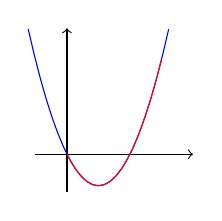
\begin{tikzpicture}[scale=0.4]
			\draw[->] (-1, 0) -- (4, 0);
			\draw[->] (0, -1.2) -- (0, 4);
			\draw[blue, domain=-1.23:3.23] plot(\x, \x * \x - 2 * \x);
			\draw[red, domain=0:3] plot(\x, \x * \x - 2 * \x);
		\end{tikzpicture}
		\caption{画图、描深}
		\label{fig:figure-of-a-function-and-its-domain}
	\end{figure}

	可得其最低点纵坐标为$-1$(是函数的顶点),两端点的纵坐标分别为$0$和$3$,故该函数值域为$[-1,3)$。
\end{proof}

\subsection[复合]{复合(无图)}
但是有些函数的图像你可是画不出来的,比如$y=4^x-2^{x+1}+1$。那就应该使用复合函数求值域的方法了。

如果一个函数$y=f(x)$可复合成$t=g(x)$和$y=f(t)$,那么可先求$g(x)$的值域,记为$A$。然后以$A$为定义域求$f(t)$的值域
(其中$f$、$g$均可作图)。

\subsubsection{根式复合}
\subsubsection{分式复合}

\subsection{非复合}
上面介绍了这么多的复合函数求值域的方法,虽然多,但不可能用在所有函数上。那这些无法复合函数我们就不能求出它们的值域。

但是我们非常的幸运,拿到了一个单调函数(或者说函数在定义域内单调),那还是有办法的,直接代端点就可以了。

\begin{example}
	求$y=(\frac{1}{2})^x+(\frac{1}{3})^x,x\in(-\infty,2]$的值域
\end{example}
\begin{proof}[解]
	由题意得,函数单调递减。

	$\therefore y\in[\frac{13}{36},+\infty)$
\end{proof}

\section{何为数理分析}
在前面的小节中,我们学会了求解三样东西:不等式、值域和方程。它们是数理分析的主要手段。

数理分析的基本思想:等式(即方程)用掉一个等式,可以减少一个未知数的个数(即消元),最终获得只含一个未知数的等式、代数式或不等式。

所谓的数理分析即:在正式计算前的一种预测,即将多于等式的未知数全部用掉后,在最终一个等式的情况下,未知数还剩几个:

\begin{desclist}
	\item[若只剩一个未知数] 可求值
	\item[若剩两个未知数] 则可求范围
	\item[若剩超过两个未知数] 则此题还有变数(可能是条件还没有找到,可能需要等待一个巧合,可能是双变量等等)
\end{desclist}
\[\begin{aligned}
	\begin{cases}
		f(x,y,z)=0 \\
		g(x,y,z)=0 \\
		h(x,y,z)=0
	\end{cases}&\text{可分别解得$x,y,z$}
	&\begin{cases}
		f(x,y,z)=0 \\
		g(x,y,z)=0
	\end{cases}&\text{可求$x,y,z$的范围} \\
	\begin{cases}
		f(a,b,c,d)=0 \\
		g(a,b,c,d)=0
	\end{cases}&\text{未必可解}
	&\begin{cases}
		f(x)>0 \\
		g(x)>0
	\end{cases}&\text{分别解完后求交集} \\
	\begin{cases}
		f(x,y)>0 \\
		g(x,y)>0
	\end{cases}&\text{线性规划(同向可加)}
	&\begin{cases}
		f(x,y)>0 \\
		g(x,y)=0
	\end{cases}&\text{利用$g$消元,可解$f$}
\end{aligned}\]

注意可解不等式只能含一个变量,不等式组也只能含一个变量,不等式组只是解集的交并关系,不等式不可用来消元。

多变量不等式是线性规划问题(同向可加性是最简线性规划问题)。

在有多个字母的情况下(尤其是涉及到复数),使用数理分析可快速的找到解题思路。

\chapter{函数性质}
函数能够很好的描述一样东西的变化规律,从而得出结论(从先前章节的笔记就可以看出)。但这还不够,想要深入分析,我们还是要了解更多的知识。

在本章中,你会学习一些新的函数及其图像。再依靠图像,得出函数的某些性质,并证明之。

\section{函数图像}
在初中我们学过一次函数、反比例函数以及二次函数,它们的图像就不再介绍了。如记性不好的去请教初中数学老师。

顺带提一句:下文讲述的函数的绘制方法只能画出近似的、粗略的函数图像,这种精度在绝大多数情况下是没有问题的\footnote{例外情况指方程的解的个数问题,前文已经提过。},您也应该在绝大多数情况下绘制这种图像。

对于三角函数,会在后面的“三角函数”章节提到。这里仅仅画出它们的图像而不研究其性质。

\subsection{耐克函数}
首先介绍的是耐克函数(或称对勾函数),它的解析式形如:\[y=ax+\frac{b}{x}\]

通过描点法,不难画出它的图像(如图\ref{fig:figure-of-tick-functions})。

\begin{figure}[htb]
	\centering
	\begin{subfigure}[b]{0.24\textwidth}
		\centering
		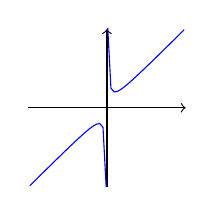
\begin{tikzpicture}[scale=0.1]
			\draw[->] (-10, 0) -- (10, 0);
			\draw[->] (0, -10) -- (0, 10);
			\draw[color=blue, domain=0.1:9.8] plot(\x, \x + 1 / \x);
			\draw[color=blue, domain=-9.8:-0.1] plot(\x, \x + 1 / \x);
		\end{tikzpicture}
		\caption{$y=1+\frac{1}{x}$}
		\label{fig:figure-of-tick-functions-a}
	\end{subfigure}
	\begin{subfigure}[b]{0.24\textwidth}
		\centering
		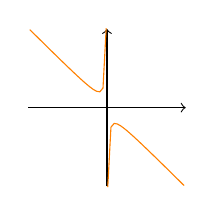
\begin{tikzpicture}[scale=0.1]
			\draw[->] (-10, 0) -- (10, 0);
			\draw[->] (0, -10) -- (0, 10);
			\draw[color=orange, domain=0.1:9.8] plot(\x, -\x - 1 / \x);
			\draw[color=orange, domain=-9.8:-0.1] plot(\x, -\x - 1 / \x);
		\end{tikzpicture}
		\caption{$y=-1-\frac{1}{x}$}
		\label{fig:figure-of-tick-functions-b}
	\end{subfigure}
	\begin{subfigure}[b]{0.24\textwidth}
		\centering
		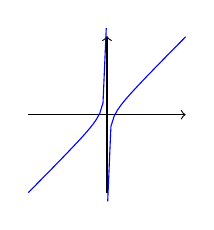
\begin{tikzpicture}[scale=0.1]
			\draw[->] (-10, 0) -- (10, 0);
			\draw[->] (0, -10) -- (0, 10);
			\draw[color=blue, domain=0.09:10] plot(\x, \x - 1 / \x);
			\draw[color=blue, domain=-10:-0.09] plot(\x, \x - 1 / \x);
		\end{tikzpicture}
		\caption{$y=1-\frac{1}{x}$}
		\label{fig:figure-of-tick-functions-c}
	\end{subfigure}
	\begin{subfigure}[b]{0.24\textwidth}
		\centering
		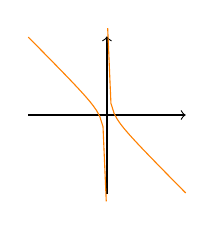
\begin{tikzpicture}[scale=0.1]
			\draw[->] (-10, 0) -- (10, 0);
			\draw[->] (0, -10) -- (0, 10);
			\draw[color=orange, domain=0.09:10] plot(\x, -\x + 1 / \x);
			\draw[color=orange, domain=-10:-0.09] plot(\x, -\x + 1 / \x);
		\end{tikzpicture}
		\caption{$y=-1+\frac{1}{x}$}
		\label{fig:figure-of-tick-functions-d}
	\end{subfigure}
	\caption{参量取不同值时耐克函数的图像}
	\label{fig:figure-of-tick-functions}
\end{figure}

然后我们可以得出耐克函数图像的性质:

\begin{itemlist}
	\item $a^+,b^+$是一、三象限的耐克函数(如图\ref{fig:figure-of-tick-functions-a})
	\item $a^-,b^-$是二、四象限的耐克函数(如图\ref{fig:figure-of-tick-functions-b})
	\item $a^+,b^-$是双增函数(如图\ref{fig:figure-of-tick-functions-c})
	\item $a^-,b^+$是双减函数(如图\ref{fig:figure-of-tick-functions-d})
\end{itemlist}

再看一眼函数图像,$a$、$b$同号时在各个象限内有极值点,接下来将推导出这个点的坐标:

\begin{proof}
	根据基本不等式得:\[ax+\frac{b}{x}\geq2\sqrt{ab}\]

	此时不等号右边即极值点的纵坐标,代入原式解方程:
	\[\begin{split}
		&ax+\frac{b}{x}=2\sqrt{ab} \\
		&ax^2-2x\sqrt{ab}+b=0 \\
		&x=\sqrt{\frac{b}{a}}
	\end{split}\]

	可以得到耐克函数在第一象限内的顶点坐标为$(\sqrt{\frac{b}{a}},2\sqrt{ab})$,其它象限只需在对应的地方添负号即可。
\end{proof}

\subsection{幂函数}
在初中我们学过了反比例函数、二次函数,它们都是幂函数的一种。其解析式为:\[y=x^a(a=\frac{p}{q}\quad p,q\in\mathbb{Z})\]

要绘制幂函数的图像,应把第一象限的图像和其余部分的图像分别绘制。

第一象限的图像如图\ref{fig:figure-of-power-function}所示。

\begin{figure}[htb]
	\centering
	\begin{subfigure}[b]{0.3\textwidth}
		\centering
		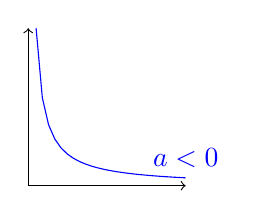
\begin{tikzpicture}[scale=0.2]
			\draw[->] (0, 0) -- (10, 0);
			\draw[->] (0, 0) -- (0, 10);
			\draw[color=blue, domain=0.5:10] plot(\x, 5 / \x) node[above] {$a<0$};
		\end{tikzpicture}
		\caption{减}
	\end{subfigure}
	\begin{subfigure}[b]{0.3\textwidth}
		\centering
		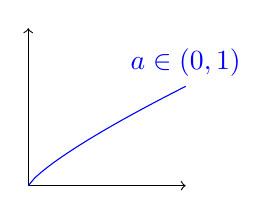
\begin{tikzpicture}[scale=0.2]
			\draw[->] (0, 0) -- (10, 0);
			\draw[->] (0, 0) -- (0, 10);
			\draw[color=blue, domain=0:10] plot(\x, \x ^ 0.8) node[above] {$a\in(0,1)$};
		\end{tikzpicture}
		\caption{缓慢增}
	\end{subfigure}
	\begin{subfigure}[b]{0.3\textwidth}
		\centering
		\begin{tikzpicture}[scale=0.2]
			\draw[->] (0, 0) -- (10, 0);
			\draw[->] (0, 0) -- (0, 10);
			\draw[color=blue, domain=0:6.81] plot(\x, \x ^ 1.2) node[right] {$a>1$};
		\end{tikzpicture}
		\caption{快速增}
	\end{subfigure}
	\caption{幂函数第一象限内的图像}
	\label{fig:figure-of-power-function}
\end{figure}

其它象限的图像可按照下面的流程绘出:
\[\begin{cases}
	\text{$q$为偶数} & \text{只有第一象限图像} \\
	\text{$q$为奇数} & \text{判断$p$}
	\begin{cases}
		\text{$p$为奇数} & \text{函数为奇函数} \\
		\text{$p$为偶数} & \text{函数为偶函数}
	\end{cases}
\end{cases}\]

\section{反函数}
我们知道,将某一个特定的值代入函数的自变量(即$x$)可以求出因变量(即$y$)的值。那已知$y$求$x$呢?解方程即可。

那我们就可以更进一步,直接用$y$来表示$x$,那就是\textbf{反函数}了。

由于函数需要$x$对应一个$y$,所以我们可以得到$x$、$y$\textbf{一一对应}是反函数存在的充要条件。

\section{导数}
在之前的笔记中,单调性可以描述一个函数在某一区间的增减性。但它具有局限性:我们只能知道一个大体的情况(增、减或非单调),而不能知道它的具体增减量为何。

再设想一下:我们通过描点法画出了函数上的几个点,要使用曲线连接把它们连接起来。由于两点之间的距离比较大,我们可能会画出几种不同的图像(如图\ref{fig:two-different-function-figure})。

\begin{figure}[htb]
    \centering
    \begin{tikzpicture}
        \draw[->] (-2, 0) -- (2, 0);
        \draw[->] (0, -2) -- (0, 2);
        \draw[color=blue,domain=-2:2] plot (\x, -0.55*\x*\x+0.15*\x+1.2);
		\filldraw (-1, 0.5) circle (1pt) (0, 1.2) circle (1pt) (1, 0.8) circle (1pt);
    \end{tikzpicture}
    \begin{tikzpicture}
        \draw[->] (-2, 0) -- (2, 0);
        \draw[->] (0, -2) -- (0, 2);
        \draw[color=orange,domain=-1.26346:1.2423] plot (\x, 2.1667*\x*\x*\x-0.55*\x*\x-2.01667*\x+1.2);
		\filldraw (-1, 0.5) circle (1pt) (0, 1.2) circle (1pt) (1, 0.8) circle (1pt);
    \end{tikzpicture}
    \caption{描点法作出的两种截然不同的图像}
    \label{fig:two-different-function-figure}
\end{figure}

当然,我们可以描更多的点作更精确的图像,那可就无穷无尽了。

不过如果我们知道一些更详细的函数性质,比如说函数只有一个递增区间和一个递减区间,那么就可以知道左图更符合目标函数的图像。

综上可以看出:过去研究的函数及其性质存在不足。故需要引入新的东西,叫做\textbf{导数}\footnote{“导数”即导函数,函数某一点处的斜率称为“导数值”。}。

求函数某一点导数值的公式如下\footnote{极限的求法不是重点,故不介绍。所以请自己领悟(笑)}:\[f'(x_0)=\lim_{h\rightarrow 0}\frac{f(x_0+h)-f(x_0)}{h}\]其几何意义是$y=f(x)$在点$P(x_0, f(x_0))$处切线的斜率。

知道了函数某一点处的斜率,我们就可以根据下面的公式:\[y-f(x_0)=f'(x_0)(x-x_0)\]求出该点的切线方程。

\begin{example}
	利用导数的定义求$y=x^2$在$x=1$处的导数$f'(1)$,并求此函数在$x=1$时的切线方程
\end{example}
\begin{proof}[解]
	先套公式得导数值:\[f'(1)=\lim_{h\rightarrow 0}\frac{(1+h)^2-1}{h}=\lim_{h\rightarrow 0}h+2=2\]

	然后求得切线方程:\[y-1=2(x-1)\Rightarrow y=2x-1\qedhere\]
\end{proof}

将求导数值的公式稍作修改,就可以得到导函数的定义求法:\[f'(x)=\lim_{h\rightarrow 0}\frac{f(x+h)-f(x)}{h}\]

\begin{example}
	用定义求$f(x)=x^2$的导函数
\end{example}
\begin{proof}[解]
	这道例题很简单,只需带入公式即可:\[f'(x)=\lim_{h\rightarrow 0}\frac{(x+h)^2-x^2}{h}=\lim_{h\rightarrow 0}2x+h=2x\qedhere\]
\end{proof}

\subsection{求导函数}
在上文,我们求出了$y=x^2$的导函数。使用定义求法当然可以求出很多函数的导函数。不过由于知识水平有限,更多函数的导函数是算不出来的,所以下面这个列表整理了基础函数的导函数:

\begin{desclist}
	\item[多项式函数] $(C)'=0$;$(x^a)'=ax^{a-1}$
	\item[指对函数] $(e^x)'=e^x$;$(\ln x)'=\frac{1}{x}$
	\item[三角函数] $(\sin x)'=\cos x$;$(\cos x)'=-\sin x$
\end{desclist}

此外,导数值为$0$的点称为函数的驻点。

\begin{example}
	求$y=\sin x$的导函数及其驻点
\end{example}
\begin{proof}[解]
	根据基础函数的导函数得:\[y'=(\sin x)'=\cos x\]

	解方程即可得驻点:\[\cos x=0\Rightarrow x=k\pi+\frac{\pi}{2}\qedhere\]
\end{proof}

我们知道初等数学有四则运算,那导数呢?肯定有四则运算,它的运算法则如下:

\begin{desclist}
	\item[加减法] $(f\pm g)'=f'\pm g'$
	\item[数乘] $(Cf)'=C\cdot f'$
	\item[乘法] $(f\cdot g)'=f'g+fg'$
	\item[除法] $(\frac{f}{g})'=\frac{f'g-fg'}{g^2}$
\end{desclist}

\begin{quote}
	如果不按照运算法则去计算导数,而仅仅凭错误的经验,老师说不定会生气到想要揍你哦(苦笑)
\end{quote}

咳咳,回到正题:注意四则运算中没有包括指数运算,不过这个是小事情,不用担心,过一会儿会介绍指数函数的求导。

\noindent\dotfill

要求对数函数的导数,要先利用换底公式:$\log_ax=\frac{\ln x}{\ln a}$,然后使用指对函数的求导公式求导:
\[(\log_ax)'=\frac{1}{x\ln a}\]

\begin{example}
	求$y=\log_2x$的导数
\end{example}
\begin{proof}[解]
	运用换底公式和导数的除法得:
	\[\begin{aligned}
		y'&=(\log_2x)'=(\frac{\ln x}{\ln2})' \\
		  &=(\frac{1}{\ln2}\cdot\ln x)'=\frac{1}{x\ln2}
	\end{aligned}\]

	注意$\frac{1}{\ln2}$是一个常数,可以提出。
\end{proof}

\noindent\dotfill

求三角函数的导数,需要全部化到一倍角后利用切割化弦,全部换成$\sin$和$\cos$后利用三角函数的求导公式求导。

其它三角函数的导函数:

\[
	\begin{aligned}
		(\tan x)'&=\sec^2x \\
		(\cot x)'&=-\csc^2x \\
		(\sec x)'&=\tan x\cdot\sec x \\
		(\csc x)'&=-\cot x\cdot\csc x
	\end{aligned}
\]

\begin{example}
	求$y=\sin2x$的导函数
\end{example}
\begin{proof}[解]
	依照上述求三角函数的导函数的方法可得:
	\[\begin{aligned}
		y'&=(\sin2x)'=2(\sin x\cos x)' \\
		  &=2[(\sin x)'\cos x+\sin x(\cos x)'] \\
		  &=2(\cos^2x-\sin^2x)=2\cos2x
	\end{aligned}\qedhere\]
\end{proof}

\subsubsection{复合函数的导数}
刚刚我们求过了$y=\sin2x$的导函数,这明显太麻烦了。对于这类可以复合的函数,我们可以使用下面的方法求导。

若$y=F(x)$可复合成$u=g(x)$和$y=f(u)$,那么$F'(x)=g'(x)f'(u)$,注意最后$u$要换回$x$。

\begin{example}
	求$y=\sin2x$的导函数
\end{example}
\begin{proof}[解]
	该函数可复合成如下函数:
	\[\begin{aligned}
		&u=2x \\
		&y=\sin u \\
	\end{aligned}\]

	则该函数的导函数为:\[y'=(2x)'(\sin u)'=2\cos u=2\cos 2x\qedhere\]
\end{proof}

利用对数恒等式得到$a^x=e^{\ln a^x}=e^{x\ln a}$,然后可利用复合函数求导得指数函数的导数(这里不设例题)。其公式为:\[(a^x)'=a^x\ln a\]

\begin{example}
	求$y=2^{2x+1}$的导函数
\end{example}
\begin{proof}[解]
	公式只能求$2^x$的导数,不能求$2^{2x+1}$,所以应该使用复合函数求导。

	该函数可复合成如下函数:
	\[\begin{aligned}
		&u=2x+1 \\
		&y=2^u \\
	\end{aligned}\]

	使用乘法公式得导函数:\[y'=(2x+1)'(2^u)'=2\ln 2\cdot2^u=2\ln2\cdot2^{2x+1}\qedhere\]
\end{proof}

\subsection{利用导函数研究函数性质}
导函数反应了原函数的增减情况,我们可以使用导函数间接研究函数性质。

上面提到过,驻点是导数值为$0$的点,在这个点上函数既不增也不减。以驻点为切入点研究函数性质正合适。

高中数学涉及的函数性质有:单调性、对称性、周期性以及最值值域。求单调区间及值域是要画图的,它们可以用导数来求。

\subsubsection{单调性}
导函数嘛,本来就是表示函数斜率的变化情况的,非常适合用来求单调性。

刚刚提过,在驻点上,函数不增也不减,我们就可以认为它是单调区间的临界值。不过这样的说法不是特别准确,可否恳请阁下仔细思考下面两个命题:

\begin{enumlist}
	\item 导函数无驻点,原函数是单调函数
	\item 导函数有驻点,原函数非单调
\end{enumlist}

命题$1$显然是真的,随便想想即可得出。对于命题$2$,我们可以观察$y=x^3$的图像及其导函数$y'=3x^2$的图像:$y=x^3$是严格增函数,继续观察导函数的图像可发现此函数有驻点$x=0$。故我们得出命题$2$是假命题。

根据导函数的几何意义,$f'(x)>0$的部分是单调递增区间;$f'(x)<0$的部分是单调递减区间(不建议解不等式,太麻烦)。

不过我们可以根据导函数求出驻点和无定义点,用驻点和无定义点将定义域分成若干部分,再判断每一部分导数值的符号从而确定该部分的单调性。驻点可以合并进单调区间。

\begin{example}
	求函数$y=x^3+x^2-x-1$的单调区间
\end{example}
\begin{proof}[解]
	先求导函数:\[y'=3x^2+2x-1\]

	再求驻点:\[3x^2+2x-1\Rightarrow x=-1\text{或}\frac{1}{3}\]

	驻点将定义域分成三段,求各段导数值的符号:
	\[\begin{aligned}
		(-\infty,-1]&\quad+ \\
		[-1, \frac{1}{3}]&\quad- \\
		[\frac{1}{3},+\infty)&\quad+
	\end{aligned}\]

	最后总结单调区间:
	\[\begin{aligned}
		\text{增区间:}&(-\infty,-1]\text{和}[\frac{1}{3},+\infty) \\
		\text{减区间:}&[-1,\frac{1}{3}]
	\end{aligned}\qedhere\]
\end{proof}

\subsubsection{极值点}
存在$x=x_1$附近的邻域($x_1$左边到$x_1$右边的一个很小的区间),使该区间内其它自变量对应的函数值都不大于$f(x_1)$,称$x_1$是函数的极大值点,$f(x_1)$是极大值。

根据上述的定义,求出的极大值点只是局部极大值,不是函数的最大值。观察图\ref{fig:figure-of-quartic-function},$B$处是局部极大值点,但$A$处才是函数的最值处。

\begin{figure}[htbp]
	\centering
	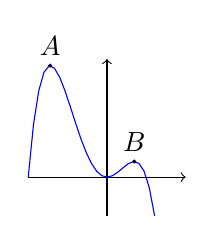
\begin{tikzpicture}[scale=0.5]
		\draw[->] (-2, 0) -- (2, 0);
		\draw[->] (0, -1) -- (0, 3);
		\draw[blue, domain=-2:1.21] plot(\x, -1 * \x * \x * \x * \x - \x * \x * \x + 2 * \x * \x);
		\filldraw (-1.443, 2.833) circle (1pt) node[above] {$A$};
		\filldraw (0.693, 0.397) circle (1pt) node[above] {$B$};
	\end{tikzpicture}
	\caption{$-x^4-x^3+2x^2$的图像}
	\label{fig:figure-of-quartic-function}
\end{figure}

和上面求单调区间一样,我们还是需要先求出导函数,然后求出驻点,再根据驻点附近$f'(x)$的符号判断此驻点是否为最值点。

\subsubsection{研究函数图像}\label{sec:mathsAnalysis-derivative-studyPorpertyOfFunction-figureOfFunction}
在上文,我们知道了如何用导函数求出原函数的单调区间以及极值点,这足以画出一个函数图像了(当然是不太精确的图像,但是关键的部分已经具备)。它常常用来求最值值域问题。

画函数图像嘛,也没啥技巧。端点和极值点描一下,根据单调性把这些点连起来就是了。

\begin{example}
	用一张长宽都是$10$的正方形白纸,四周分别减去一块变长为$x$的正方形,折成一个简易垃圾桶,求该简易垃圾桶的最大容积
\end{example}
\begin{proof}[解]
	先列出容积$V$关于$x$的函数解析式,并标明定义域:\[V=x(10-2x)^2=4x^3-40x^2+100x(0<x<5)\]

	很显然,我们画不出它的图像,那么就应该使用导函数了:\[V'=12x^2-80x+100\]

	求出驻点:\[12x^2-80x+100=0\Rightarrow x=\frac{5}{3}\text{或}5\]

	这样定义域被分成$2$段:$[0,\frac{5}{3}]$和$[\frac{5}{3},5]$。通过计算各段的导数值可知函数在$[0,\frac{5}{3}]$上单调递增;在$[\frac{5}{3},5]$上单调递减。

	然后算出图像分别经过点$(0,0)$、$(\frac{5}{3},\frac{2000}{27})$和$(5,0)$,即可作出如图\ref{fig:drawing-figure-with-derivative}的函数图像,可得其最大值为$\frac{2000}{27}$。

	\begin{figure}[htbp]
		\centering
		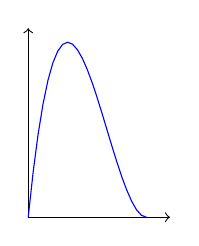
\begin{tikzpicture}[scale=0.3]
			\draw[->] (0, 0) -- (6, 0);
			\draw[->] (0, 0) -- (0, 8);
			\draw[blue,domain=0:5] plot(\x, 0.4 * \x * \x * \x - 4 * \x *\x + 10 * \x);
		\end{tikzpicture}
		\caption{通过导函数画出来的函数图像}
		\label{fig:drawing-figure-with-derivative}
	\end{figure}

	$\therefore$该简易垃圾桶的最大容积为$\frac{2000}{27}$。
\end{proof}

\end{document}
